\subsection{Timescale}
\begin{figure}[h]
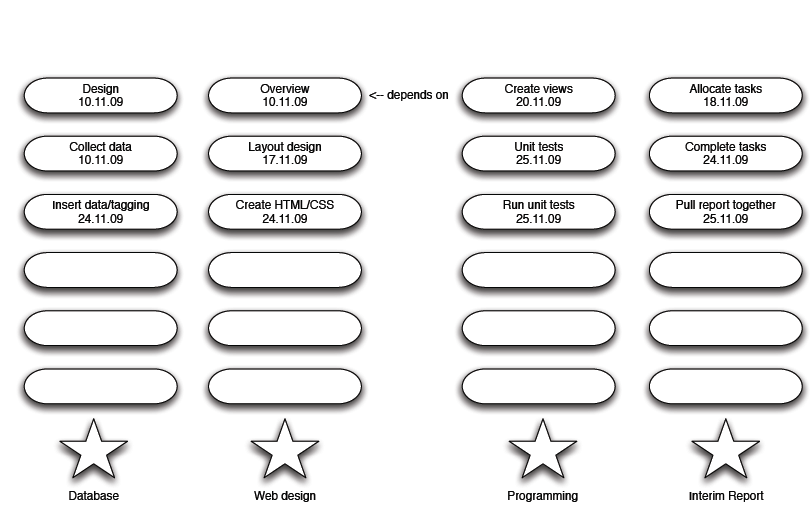
\includegraphics[width=0.9\textwidth]{timescale}
\caption{Project Timescale}
\label{fig:time_scale}
\end{figure}

The project timeline can be decomposed to 4 key deadlines:
\begin{enumerate}
	\item Interim report submission (04/12/2009)
	\item Final report due (01/04/2010)
	\item Open day (05/05/2010)
	\item Presentation day (07/05/2010)

\end{enumerate}



Since our group is adopting the methodology of prototyping, a milestone chart is to be made for each of the three versions which conform to the above deadlines. Above is the detailed timeline of the version 1 prototype expressed as a project milestone chart (Fig~\ref{fig:time_scale}).
Each oval represents a downward progression to the milestones, represented by stars. The dates represent the deadlines that the group deemed appropriate for each progression. The group decided early on to plan out the web and database design together, which is essentially “the meat” of our project. Thereafter, tasks will be allocated to each member where the individual heads of the project will take charge of their respective domains. Deadlines of specific tasks are as elucidated by the above. Notice that version 1 is to be completed before the deadline for the interim report which exemplifies the fact that our chart takes into account the major deadline dates.

Due to the dynamic nature of our project, it was decided that further milestone charts will be designed as we progress from the completion of one version to another. Moreover, it is unwise to have planned out charts for future versions before even acquiring a feel of the project.
\newpage

 
